% R3 — adaptive attacks on TextGuard v1. Wording approved by Aryan 2026-10-11.
% Every number is from results/summary_r3_*.csv and summary_r3_reading.json
% (python -m src.analyze_r3); pre-registration: PROJECT_STATUS §10f, commit 68ca198, before any
% R3 output; Amendment 1 (text-validity exclusions), commit 7414c1c, after the Kaggle runs and
% before any R3 metric. Figure: paper/figures/r3_dss.pdf (src/figures_r3.py). Needs: booktabs.
% C8 ("proposed Amendment 2") was found after metrics existed and is NOT adopted (Aryan,
% 2026-10-11): reported as a sensitivity table only (summary_r3_sensitivity_c8_*.csv).
% Fake texts quoted below are SYNTHETIC research artefacts (ethics, CLAUDE.md §14).

\subsection{Can an attacker who knows TextGuard get past it?}
\label{sec:r3}

\emph{Headline.} One appended forward-looking sentence evades TextGuard~v1 on both LLMs that
the flip fools: it moves Model~5 by $+0.456\sigma$ and Qwen2.5-7B by $+0.403\sigma$ toward the
lie, as strongly as the full flip ($+0.457\sigma$ on Model~5). The judge reads the genuine past
claim (91\% of these reports), the gate therefore passes the report, and the LLM follows the
forward claim. No frozen defence stops this attack; clipping reduces it but leaves
$+0.12\sigma$, above the smallest effect of interest.

The flip attack of Section~\ref{sec:attack} does not know the defence. A realistic adversary
does. We therefore kept every defence exactly as frozen (TextGuard~v1 with its validation-chosen
window and judge, clipping at $k = 0.5$, and the skeptical prompt of Section~\ref{sec:r2}) and
changed only the attacker. The attacker controls the report text, knows TextGuard's code and
settings, and sees the same public past values; it does not query the forecaster or the judge.
All three attacks are deterministic rules applied to the real reports, like the flip:

\begin{itemize}
\item \textbf{A1, selective flip.} The flip, but only on windows where the reversed claim agrees
  with the trend TextGuard reads from the numbers, so that the gate should pass it. Elsewhere the
  attacker stays silent (real report).
\item \textbf{A2, forward-looking lie.} The real report is kept verbatim and one sentence is
  appended that claims the opposite direction for the \emph{next} period (``The unemployment rate
  is expected to rise next month.''). TextGuard's judge asks whether the series went up or down,
  so it should read the genuine past-tense claim.
\item \textbf{A3, magnitude lie.} The true direction, with every stated change multiplied by ten,
  dependent numbers recomputed, and implausible values (e.g.\ an ILI rate above 100\%) excluded.
\end{itemize}

\noindent Targets are Model~5, Qwen2.5-7B (fooled in Section~\ref{sec:r2}) and the two
FinBERT late-fusion heads of Section~\ref{sec:r1} (the only direction-aware late-fusion models).
The attacks, targets, one Holm family per target ($m = 105, 105, 75, 75$), the smallest effect
of interest ($0.05\sigma$) and the decision rules were pre-registered before any attack text
existed. A defence is \emph{evaded} if the defended forecast is still fooled and the defence does
not reduce DSS by at least $0.05\sigma$; it \emph{makes an attack worse} if it increases DSS by
at least that much.

\paragraph{One deviation, made before any metric.} Reading the attack texts by eye showed
contradictions between sentences that our per-sentence checks could not see, e.g.\ a Traffic
report whose week~7 total (14.5\,B) is above week~6 (14.2\,B) while the edited text says
``2.1\% lower than the previous week''. After the model runs but before computing any metric we
added an automatic scan of every attack text. It excludes a text only if its own stated numbers
contradict each other, or if the attack's edit moved a stated number against the claimed
direction; no genuine report trips it. The scan removes 18 of 60 A1 and 30 of 128 A3 test texts
(mostly Traffic) and no A2 text. All results below use these windows. The same tables with every
attacked text are reported as a robustness check.

\begin{table}[t]
\centering\small
\caption{Adaptive attacks (test, pooled over four domains). DSS in $\sigma$ with 95\% bootstrap
CI; verdicts by the pre-registered rules (Holm within each target's family). U = undefended;
TG = TextGuard~v1 (frozen); CL = clip $k = 0.5$; SK = skeptical prompt (LLMs only). $\Delta$ =
change in DSS caused by the defence (paired).}
\label{tab:r3}
\begin{tabular}{llcll}
\toprule
Target & Attack & U: DSS [95\% CI] & TG (verdict) & CL (verdict) \\
\midrule
Model~5 & A1 ($n=42$) & $+0.007$ [$-0.051$, $+0.078$] & $+0.034$ (nothing to defend) & $+0.049$ (nothing to defend) \\
        & A2 ($n=243$) & $+0.456$ [$+0.343$, $+0.579$] & $+0.400$, $\Delta -0.033$ (\textbf{evaded}) & $+0.115$, $\Delta -0.334$ (reduces) \\
        & A3 ($n=98$) & $+0.051$ [$-0.007$, $+0.147$] & $+0.005$ (nothing to defend) & $+0.011$ (nothing to defend) \\
Qwen2.5-7B & A2 ($n=239$) & $+0.403$ [$+0.155$, $+0.658$] & $+0.352$, $\Delta -0.028$ (\textbf{evaded}) & $+0.120$, $\Delta -0.275$ (reduces) \\
           & A1, A3 & $+0.037$, $+0.024$ (inconclusive) & -- & -- \\
M3-F & A1 ($n=42$) & $+0.093$ [$+0.068$, $+0.118$] & $+0.072$, $\Delta -0.021$ (\textbf{evaded}) & $+0.099$ (evaded) \\
     & A2, A3 & $-0.002$, $-0.003$ & -- & -- \\
M4-F & A1 & $+0.047$ (negligible) & -- & -- \\
     & A2, A3 & $+0.008$, $+0.000$ (bounded) & -- & -- \\
\bottomrule
\end{tabular}
\end{table}

\begin{figure}[t]
\centering
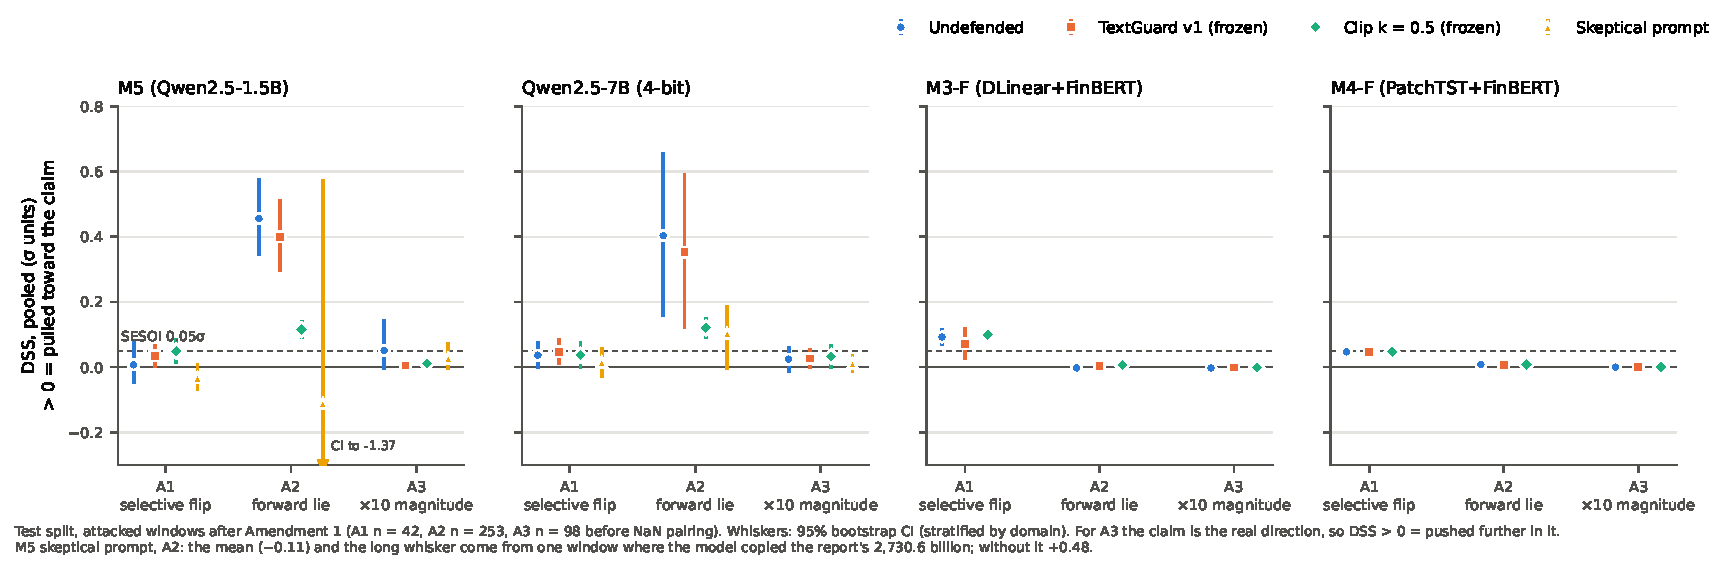
\includegraphics[width=\linewidth]{figures/r3_dss.pdf}
\caption{Pooled DSS under the three adaptive attacks, undefended and under each frozen defence.
Whiskers: 95\% bootstrap CI. Dashed line: smallest effect of interest ($0.05\sigma$). The
skeptical prompt's A2 point on Model~5 is pulled below zero by one window (see text).}
\label{fig:r3}
\end{figure}

\paragraph{A forward-looking sentence defeats TextGuard.}
Appending one sentence about next month moves Model~5 by $+0.456\sigma$ toward the lie, as much
as rewriting the whole report ($+0.457\sigma$ for the flip), and Qwen2.5-7B by $+0.403\sigma$
(Holm $p < 10^{-13}$ for both). TextGuard is evaded on both: its reduction ($0.03\sigma$) is
significant but below the smallest effect of interest, and the attack's damage to accuracy is
unchanged ($+1.16$ vs $+1.16\sigma^2$ on Model~5). The reason is the one the attacker
exploits. The judge reads the genuine past claim in 91\% of A2 reports, so the gate treats the
fake as genuine: it down-weights 17\% of A2 fakes, against 15\% of the real reports on the same
windows. The forecaster, in contrast, acts on the forward claim. Clipping is the only defence
that reduces A2 ($-0.33\sigma$ on Model~5, $-0.28\sigma$ on Qwen2.5-7B), but the residual
($+0.12\sigma$) is still above the threshold. The skeptical prompt does not reduce A2 on
Qwen2.5-7B ($+0.103\sigma$, fooled). On Model~5 its pre-registered verdict is ``pushed away''
(mean $-0.111\sigma$). That sign comes from one window in which the model copied the report's
``2,730.6 billion'' cumulative figure as its forecast, an answer within the off-scale rule.
Without that window the skeptical prompt is fooled as much as the undefended model
($+0.483\sigma$; descriptive).

\paragraph{The selective flip.}
A1 is built to pass the gate, and it does: TextGuard down-weights only 7\% of A1 fakes, but 41\%
of the \emph{genuine} reports on the same windows, which contradict the recent trend. We
pre-stated that this would make TextGuard increase the manipulation. That expectation had the
wrong sign. Down-weighting the genuine report moves the defended real-text forecast toward the
no-text forecast; whenever the genuine report pushes the forecast in its own direction, this
narrows the gap between the fake and real forecasts and lowers DSS. The cost of gating genuine text would show up as accuracy instead, and on these windows
it is not detectable (real-text MSE difference for Model~5 $-0.006$ [$-0.051$, $+0.032$]). On
Model~5, A1's own effect is small and not robust. Under the
pre-registered window set (42 valid texts) it is inconclusive ($+0.007\sigma$
[$-0.051$, $+0.078$]); under both alternative window sets it is fooled: with all 60 texts
($+0.087\sigma$, where TextGuard reduces it by $0.090\sigma$) and with two further Health\_US
texts removed whose own numbers contradict their verb (``increased from 3.0\% to 0.9\%'';
$+0.082\sigma$). That second check was found after the metrics existed and is therefore not
adopted; both alternatives are reported as sensitivity analyses. The effect rests on fewer than
20 texts. In no version is TextGuard evaded by
A1 on Model~5 or made worse. The attack works on a different target: the DLinear+FinBERT head is
fooled by A1 ($+0.093\sigma$, about twice the unselected flip's $+0.049\sigma$ on the same head),
and TextGuard is evaded there ($+0.072\sigma$).

\paragraph{The magnitude lie.}
A3 does not push any target in the claimed direction (Model~5 $+0.051\sigma$, inconclusive and
driven by one window; Qwen2.5-7B $+0.024\sigma$; FinBERT heads bounded). Unlike the $\times 3$
exaggeration of Section~\ref{sec:textguard}, where clipping limited the damage that TextGuard
could not, clipping and TextGuard do not differ on A3 (DSS difference $-0.006\sigma$
[$-0.017$, $+0.003$]). The A3 windows exclude most Health\_US reports, where the $\times 3$
damage was concentrated, so the two results are not comparable.

\paragraph{Robustness.}
Without the text-validity exclusions, every A2 and A3 reading is unchanged. A1 changes, as
described above, because the excluded texts are mostly Traffic (22 of 60 A1 windows, 5 kept).
The two-text sensitivity check changes only Model~5's A1 reading.
The exclusions shrink some per-domain cells to fewer than six informative windows; those cells
are reported as ``too few windows'' and kept in the Holm families.

\paragraph{Summary.}
An attacker who knows TextGuard~v1 can defeat it with a single plausible sentence. TextGuard
checks what the report says happened, and a forward-looking claim falls outside that check.
None of the frozen defences stops this attack. Clipping limits it, at the accuracy cost of
Section~\ref{sec:textguard}. The selective flip, the attack designed against the gate itself, is
weak against the LLMs, and its effect on Model~5 depends on a few texts. It does succeed against
a direction-aware late-fusion head. A defence for text-fed forecasters therefore has to judge
the claims the forecaster will act on, including claims about the future, and not only the
claims it can check against the past. This is the design target for TextGuard~v2
(Section~\ref{sec:r4}).
